\documentclass{article}
\usepackage{icmc,amsmath}
\usepackage{graphicx}
\usepackage{url}
\usepackage[utf8x]{inputenc}
\usepackage[T1]{fontenc}
\usepackage[english]{babel}
\usepackage{color}
%\usepackage[htt]{hyphenat}
\usepackage{times}
%\usepackage{babelbib}

\hyphenation{e-du-ca-ci-\'on}

\title{Rameau: A System for Automatic Harmonic Analysis}

\oneauthor
  {Pedro Kröger, Alexandre Passos, Marcos Sampaio, Givaldo de Cidra}
  {Genos---Computer Music Research Group\\ School of Music
   \\ Federal University of Bahia, Brazil \\
  \url{{pedro.kroger,alexandre.tp,mdsmus,givaldodecidra}@gmail.com}}

\newcounter{notacounter}

\newcommand{\nota}[1]{
  \addtocounter{notacounter}{1}
  \textcolor{red}{[nota \arabic{notacounter}: #1]}
}


\begin{document}
\graphicspath{{figs/}{data/}}
\maketitle

\begin{abstract}
%The abstract should be placed at the top left column and should contain
%about 150-200 words.

  Automated harmonic analysis is an important and interesting music
  research topic. Although many researchers have studied solutions to
  this problem, there is no comprehensive and systematic comparison of
  the many techniques proposed.

  In this paper we present Rameau, a framework for automatic harmonic
  analysis we are developing. With Rameau we are able to reimplement
  and analyze many previous techniques. We found Tsui's
  \cite{tsui:harmonic} and Pardo and Birmingham's
  \cite{pardo.ea:automated-report} algorithms promising, while
  Temperley and Sleator's \cite{temperley.ea:modeling} is too brittle
  and imprecise. 

  We also present a numeric codification for tonal music with
  interesting properties, such as easy transposition, preservation of
  enharmonic information and easy conversion to and from standard
  pitch-class notation.

\end{abstract}

\section{Introduction}
\label{sec:introduction}

In music, harmonic analysis is the study of vertical sonorities and
their connections, and is paramount to the understanding of tonal
compositions. The analyst may find the chord roots, label
sonorities with proper chords names (such as ``A minor''), and
identify their relationships using roman numerals.

Harmonic analysis by computer is an important, challenging, and
interesting music research topic. It is challenging because the
musical material has a large variety of information such as timbre,
notes, rhythm, dynamics, harmony, and because music unlike image is not a
linear process \cite{mouton.ea:numeric}. The harmonic changes in a choral
texture, where usually all notes in all voices begin and finish at the
same time, are obvious. However, chords are occasionally arppeggiated,
incomplete, and intertwined with non-harmonic tones. These things
contribute to increase considerably the complexity of analysis
\cite{pardo.ea:automated}.

There are many practical applications for automatic music analysis,
such as arranging, detection of possible logical mistakes in scores,
database search, automatic accompaniment generation, and statistical
analysis of musical styles for automated composition
\cite{pardo.ea:algorithms,temperley.ea:modeling}. Computer-based
harmonic analysis is also important because it can bring new insights
in music theory, in the same way the use of computer in vision and
problem solving has brought new insights in these areas
\cite{temperley.ea:modeling}.

Although many harmonic analysis algorithms have been proposed, no
single framework for comparing them has been developed. Every
comparison we found in literature (\cite{pardo.ea:automated,
  barthelemy.ea:figured, tsui:harmonic, taube:automatic,
  illescas.ea:harmonic}) is based solely on published examples, which
are not a very statistically representative sample. Pardo and
Birmingham \cite{pardo.ea:automated} state that ``no researchers have
published statistical performance results on a system designed to
analyze tonal music''. In this paper we will present Rameau, a
framework for automatic harmonic analysis of Western tonal music
developed as an attempt to solve this problem.

We have implemented ten algorithms for harmonic analysis in the
framework and will present in this work a preliminary evaluation of
nine of them using a corpus of 140 Bach chorales from the 371 in the
Riemenschneider edition \cite{bach:371}. Rameau automatically compares
the answers return by the algorithms with answer sheets prepared by
musicians. Since we currently have answer sheets for only 140
chorales, that will be the music corpus used in this paper, although
rameau can analyze all 371. While some algorithms are heavily based on
previous research, other approaches, like our usage of decision trees,
are new. Another significant difference between our approach and the
others found in the literature is the evaluation of performance using
precision and recall.

\section{The problem of automated harmonic analysis}
\label{sec:problem}

The problem of automated harmonic analysis may better be understood if
we divide it into four sub-problems.

The first problem is pitch spelling. If sharps and flats are not
distinguished the program may have problems whenever enharmonic
information is relevant. Most systems either ignore this problem or
develop a pitch speller \cite{temperley.ea:modeling}. Most harmonic
analysis software, with the notable exception of MusEs
\cite{pachet.ea:representing} and the system described in
\cite{illescas.ea:harmonic}, uses input formats that lose enharmonic
information.

The second problem, the segmentation problem
\cite{pardo.ea:automated}, is to determine what are the vertical
sonorities in a piece of music and group these sonorities in
harmonically significant segments, or chord-spans. The main reason for
segmentation's complexity is that the number of possible segmentations
of a piece is roughly an exponential function of its length,
impossibilitating a thorough evaluation of all possibilities
\cite{pardo.ea:algorithms}.

The third problem is labeling segments with chord names. Not every
segment forms a chord, some will consist solely of non-chord tones and
other melodic information. Labeling a segment with a chord might
require contextual information, which complicates the matter a bit,
difficulting local decisions. Still, over 80\% of accuracy is possible
ignoring context (see section \ref{sec:analysis-results}).

The last problem is finding the main key and the modulations of the
piece and assigning a tonal function to each chord.

\section{Numeric codification for tonal music}
\label{sec:codificacao-jamary}

The pitch-class notation, or some variation such as MIDI, is probably
the most used way to numerically represent pitch. The main problem
with this notation is the loss of enharmonic spelling. In this section
we will revise three notations created independently by Brinkman,
Hewlett, and Oliveira \cite{brinkman:binomial, hewlett:base-40,
  oliveira:busca} to address this problem. For the sake of simplicity
we will refer to them as binomial, base-40, and base-96, respectively.

In the binomial notation notes are represented as tuples in the form
of \texttt{<pc,nc>}, where \texttt{pc} stands for pitch-class (0 to
11) and \texttt{nc} for note-class (0 to 7). Note-class 0 means the
note is written as accidentals over C, 1 represents accidentals over
D, and so on. For example, C$\sharp$ is represented as \texttt{<1,0>},
D$\flat$ as \texttt{<1,1>}, D$\sharp$ as \texttt{<3,1>}, and C$\flat$
as \texttt{<11,0>}. In this last example 11 represents the pitch-class
of the note and 0 indicates how it will be spelled. The binomial
notation also allows a packaged representation using only single
numbers, where the pitch-class is multiplied by 10 and added to the
note-class. For example, C$\sharp$ becomes 10 and D$\flat$ 11.

Unlike the binomial notation, the base-40 notation uses only single
numbers. The octave is divided linearly in 40 notes from C$\flat\flat$
to B$\sharp\sharp$. Table \ref{tab:base40} shows a few notes in this
system.

\begin{table}
  \centering
  \begin{tabular}{l|l}
    note & code \\
    \hline
    c$\flat\flat$ & 1 \\
    c$\flat$ & 2 \\
    c & 3 \\
    c$\sharp$ & 4 \\
    c$\sharp\sharp$ & 5 \\
    -- & 6 \\
  \end{tabular}
  \caption{A few notes in the base-40 notation}
  \label{tab:base40}
\end{table}

The base-96 notation is simple, elegant, and overcomes a few
shortcomings in both the binomial and base-40 notations. As the
original publication of the base-96 notation is available only in
Portuguese, we will describe it here, comparing it with the other
two. 

The base-96 is also a single number notation. It has all the qualities
of the base-40 notation with some additional advantages. Table
\ref{tab:jama-notas} shows how notes are encoded. In this notation the
intervals are invariant under most transformations, such as inversion,
transposition, etc. Table \ref{tab:jama-intervalos} shows the coding
for the intervals. The first column indicates the interval name; P, M,
m, d, A for perfect, major, minor, diminished, and augmented,
respectively. The letters before d and A indicate the quantity of the
interval. For instance, tA is triple-augmented.

\begin{table}
  \centering
  \begin{tabular}{l|lllllll}
               & c & d& e& f& g& a& b \\
    \hline
    7$\flat$   &   & 7&21&  &  &62&76 \\
    6$\flat$   & 90& 8&22&35&49&63&77 \\
    5$\flat$   & 91& 9&23&36&50&64&78 \\
    4$\flat$   & 92&10&24&37&51&65&79 \\
    3$\flat$   & 93&11&25&38&52&66&80 \\
    2$\flat$   & 94&12&26&39&53&67&81 \\
    $\flat$    & 95&13&27&40&54&68&82 \\
    $\natural$ &  0&14&28&41&55&69&83 \\
    $\sharp$   &  1&15&29&42&56&70&84 \\
    2$\sharp$  &  2&16&30&43&57&71&85 \\
    3$\sharp$  &  3&17&31&44&58&72&86 \\
    4$\sharp$  &  4&18&32&45&59&73&87 \\
    5$\sharp$  &  5&19&33&46&60&74&88 \\
    6$\sharp$  &  6&20&34&47&61&75&89 \\
    7$\sharp$  &   &  &  &48&  &  &   \\
  \end{tabular}
  \caption{Notes in the base-96 notation}
  \label{tab:jama-notas}
\end{table}

\begin{table}
  \centering
  \begin{tabular}{l|llllllll}
    & 1$^{st}$& 2$^{nd}$& 3$^{rd}$& 4$^{th}$& 5$^{th}$& 6$^{th}$& 7$^{th}$& 8$^{th}$ \\
    \hline
    sd  &  & 7&21&35&49&62&76&90 \\
    qd  &  & 8&22&36&50&63&77&91 \\
    qd  &  & 9&23&37&51&64&77&92 \\
    td  &  &10&24&38&52&65&78&93 \\
    dd  &  &11&25&39&53&66&79&94 \\
    d   &  &12&26&40&54&67&80&95 \\
    m   &  &13&27&  &  &68&82&   \\
    P   & 0&  &  &41&55&  &  &96 \\
    M   &  &14&28&  &  &69&83&   \\
    A   & 1&15&29&42&56&70&84&   \\
    dA  & 2&16&30&43&57&71&85&   \\
    tA  & 3&17&31&44&58&72&86&   \\
    qA  & 4&18&32&45&59&73&87&   \\
    qA  & 5&19&33&46&60&74&88&   \\
    sA  & 6&20&34&47&61&75&89&   \\
    oA  &  &  &  &48&  &  &  &   
  \end{tabular}
  \caption{Intervals in base-96 notation}
  \label{tab:jama-intervalos}
\end{table}

The base-96 notation works for up to seven flats and sharps, which is
more than enough for tonal music. This system is compatible with the
pitch-class system (modulo 12): in the base-96 notation G = 55, and
the result of 55 mod 12 is 7, representing G in the pitch-class
notation. 

The problem with the base-40 notation is that it does not work with
more than two accidentals. For example, the interval between
C$\flat\flat$ and C$\sharp\sharp$ (a quadruple augmented unison) has
the same value (6) as diminished second. On the other hand, in the
base-96 notation this interval can be correctly computed.

The main problem with the binomial notation is that operations that
are (and should be) simple become complex. In both base-40 and base-96
notations, transposition is as simple as adding an index to a note,
while in the binomial system requires two different operations (mod
and div) besides the addition. Its packaged representation is supposed
to simplify things, but as an example, transposition becomes something
like:

\begin{eqnarray}
10\times((a \div 10 + B \div 10) \mod 12)\; + \nonumber \\
((a \mod 10 + B \div 10) \mod 7)
\end{eqnarray}

To do anything non-trivial, like interval-class vectors, yet extra
work has to be done, increasing complexity.

We believe the base-96 codification is a very nice form of describing
tonal music numerically and it should be more known among researches
and developers. For these reasons we have adopted it, although no
algorithm implemented in rameau at present makes direct use of it,
since they are reimplementations of algorithms designed by their
original authors expecting pitch classes as input.
% \nota{jama: o que você quer dizer?
%  Talvez confundindo o PCN--que espera pitch classes--com o
%  Objnota--que espera qualquer "coisa"?}

\section{The Rameau Framework}
\label{sec:system}

To properly study, understand and compare algorithms for automated
harmonic analysis we have designed and implemented a framework,
Rameau, that should enable us to

\begin{enumerate}
\item compare results precisely and reproducibly with manual analysis
  of a large corpus of music;
\item allow algorithms to access detailed information in the input score,
  such as enharmonic differences, meter, etc.; and
\item easily develop new algorithms, test existing ones, and precisely
  compare the results.
\end{enumerate}

Reimplementing existing algorithms in Rameau allows us to easily
evaluate their accuracy, study their errors and compare their merits
and flaws. We are unaware of any systematic comparison of different
approaches to harmonic analysis, similarly to what Gomez and Herrera
\cite{gomez.ea:song} do for tonality recognition.

Rameau is written in Common Lisp and currently runs on the Steel Bank
Common Lisp \cite{team:sbcl} and CMUCL \cite{maclachlan:cmucl}
compilers and the Clisp \cite{haible.ea:clisp} interpreter on the
GNU/Linux and Microsoft Windows operating systems. Increased
portability is one of our goals.

\subsection{Architecture}
\label{sec:architecture-and-api}

The architecture of the Rameau framework is simple. First, a score is
parsed into a list of notes, which is then split into a list of
sonorities. Then, these sonorities are sent to each algorithm for
analysis. The analysis results and their comparison with the answer
sheets are then output either textually or as an annotated score, as
in figures \ref{fig:coral-12} and \ref{fig:coral-54}.

The algorithms used for analysis are implemented using a very simple
Common Lisp API. To implement an algorithm it is only necessary to
place a lisp file in a special directory and call the
\texttt{register-algorithm} function inside that file, specifying the
algorithm's name, an analysis function and a comparison function as
parameters. The input to the analysis function is a list of
sonorities. In Rameau, sonorities are lists of notes, each note
specifying its onset time, duration, octave and pitch. The output is a
list of either chords or non-chord tones, one for each input
sonority. The comparison function is responsible for determining which
parts of the chord are to be considered when assessing correctness of
the analysis. This is necessary because, for example, Temperley and
Sleator's\cite{temperley.ea:modeling} algorithm does not identify a
chord's mode. Rameau provides a few possible comparison functions for
easy usage. Chords are represented internally as structures that may
have a root, a mode, a seventh, a bass, and other additions. The
framework also provides a rich library to deal with common musical
operations.

Using this API we have currently implemented:

\begin{enumerate}
\item a subset of the algorithm described in \cite{pardo.ea:algorithms}
  (ignoring, for now, segmentation), 
\item a work-in-progress port of the algorithm described in
  \cite{temperley.ea:modeling}, 
\item four neural networks (using the Fann \cite{nissen:fann}
  library) roughly similar to some described in
  \cite{tsui:harmonic}, and
\item four decision trees modeled after the neural networks (using code
  from \cite{mitchell:machine}).
\end{enumerate}

Rameau's source code is publicly available, under a GNU GPL
\cite{fsf:gpl} license, in a git \cite{baudis:git}
repository at \url{git://genos.mus.br/rameau.git} and for
visualization at \url{git.genos.mus.br/?p=rameau.git}.

\subsection{The interface}
\label{sec:analysis-output}

Rameau is a command line program, although a GUI version is planned.
The user can select the chorales to be analyzed and specify the
algorithms for the analysis. The output shows a table with the
partition number, the correct analysis for each sonority (taken from
the answer sheet) and the analysis output for each chosen algorithm.
The nice thing about this output is that it can be further processed
using regular unix tools such as grep, awk, and sed.

To simplify reading the results, rameau can output a score with the
chorale and the analysis from each algorithm chosen. The music
notation program LilyPond \cite{nienhuys.ea:lilypond} is used to
render the score.

Figure \ref{fig:coral-12} shows the result of the analysis of the
first phrase of chorale \#12. The first line shows the partition
number, the last line, the expected answer, and the lines in between,
the analysis results for the chosen algorithms. The output score shows
incorrect analysis in bold italic. Non-chord tones are notated as
``—''. It is important to remember that while some algorithms identify
chords, others identify only the root.

\begin{figure}
  \centering
  \includegraphics[scale=4]{coral-012}
  \caption{An analyzed excerpt from chorale 12, ``Puer natus in Bethlehem''}
  \label{fig:coral-12}
\end{figure}

Rameau performs the analysis of one chorale, using all nine
algorithms, in less than a half-second on a Pentium Celeron M at 1.4
GHz with 2 GB RAM linux box. All 140 chorales are analyzed and the
results compared with the answer sheet under 40 seconds.

\subsection{Test corpus}
\label{sec:test-corpus}

We are building a corpus of analyzed and digitalized Bach chorales to
use as training and test data. Bach chorales were chosen because:

\begin{enumerate}
\item they are easily analyzed. For example, the segmentation problem in
them consists simply of determining the sonorities.
\item Their chord density is high\,---\,there are many more chords per
  measure than in a symphony, for example.
\item They are canonical examples of tonal harmony.
\item There are 371 on the Riemenschneider edition, more than
  enough to train our algorithms and get precise error analysis.
\item Their texture is simple and constant. It consists basically of
  four voices forming simple triads and tetrads.
\item Although they have been widely used as examples
  \cite{taube:automatic, tsui:harmonic, illescas.ea:harmonic,
    winograd:linguistics}, no single research has analyzed all Bach
  chorales. We believe doing this will create a very useful corpus of
  harmonic information.
\end{enumerate}

We have answer sheets for 140 chorales and plan on fully incorporating
every chorale in the Riemenschneider \cite{bach:371} edition soon. The
corpus is stored in a subset of the GNU Lilypond format, from which we
generate MIDI files and typeset scores, possibly annotated with
analysis results (both our answer sheets and computer-made results).
The lilypond format was chosen because it is

\begin{enumerate}
\item easy to parse,
\item easy to read and write,
\item compact (unlike MusicXML), and
\item easy to convert from different formats (such as MIDI) to it.
\end{enumerate}

Also, lilypond itself can be used to typeset the scores and export
them to MIDI.

When the chorales are fully analyzed we plan on incorporating the
Kostka-Payne \cite{kostka.ea:tonal} corpus, Beethoven sonatas, Bach
cello suites and other pieces.

\subsection{The answer sheet format}
\label{sec:formato-dos-acordes}

The results of manual analysis performed on the chorales are stored in
a simple, flexible text format, designed to

\begin{enumerate}
\item be as close as possible to usual popular notation,
\item represent inherent ambiguities in chord, and
\item represent non-chord tones.
\end{enumerate}

The first four sonorities of the answer sheet for Bach's chorale \#1
``Aus meines Herzens Grunde'', for example, are stored as \texttt{G G
  C/E (C7+/E [b])}. Each chord symbols represents a sonority. Chords
in parenthesis represent possible interpretations of a single
sonority. Notes in brackets are non-chord tones, marking sonorities
that do not constitute chords.

This information is then used as answer sheets and training data on the
many algorithms implemented in our system.

\section{Preliminary results}
\label{sec:analysis-results}

\subsection{Pardo and Birmingham's algorithm}
\label{sec:pardo-birmingham}

The algorithm described in \cite{pardo.ea:automated} has some
interesting properties. It handles most simple examples of tonal
harmony really well, but has no clear notion, by design, of non-chord
tones, augmented chords and other possible analysis. We
have found no need, as of yet, of implementing the segmentation
algorithm, since segmentation is trivial in Bach Chorales.

The current accuracy is $66 \pm 9\%$.

\subsection{Temperley and Sleator's algorithm}
\label{sec:temperley}

We have reimplemented the algorithm used in Temperley and Sleator's
Melisma Music Analyzer and described in
\cite{temperley.ea:modeling}. We also found online their
implementation of their algorithm, but neither their program nor our
reimplementation was able to match the performance claimed in the
article. Tsui \cite{tsui:harmonic} was also unable to reproduce their
results.

The Melisma algorithm is brittle and depends on many parameters. Its
performance is orders of magnitude slower than any other we have
evaluated. Our reimplementation is also very fragile and occasionally
fails to process a chorale. Its accuracy is around $50 \pm 20\%$. The
original implementation's accuracy couldn't be computed due to
difficulties in parsing Melisma's output and matching it with our
answer sheets.  On the scores we manually matched, however, the
accuracy seems poor, as can be seen in figures \ref{fig:coral-12} and
\ref{fig:coral-54}.

\subsection{Neural networks}
\label{sec:neural-nets}

Neural networks are tools for non-linear statistical data
modeling that work by having artificial neurons exchange
information. There are many varieties of neural networks, each being
useful for a certain type of problem. Our networks are all multilayer
feed-forward neural networks, with one hidden layer each. This is the
standard model for pattern recognition \cite{russell.ea:artificial}.

\begin{figure}
  \includegraphics[]{neural-networks}
  \caption{The Simple-net}
  \label{fig:simple-net-diagram}
\end{figure}

We have currently implemented in Rameau four neural-network-based
algorithms for harmonic analysis, basing our approaches on
\cite{tsui:harmonic}. The input of our simplest algorithm,
\texttt{Simple-net}, is how many times each pitch class sounds in
a sonority (its pitch count). As output, the network activates the
neuron representing the root for that sonority (or does nothing, if
the sonority does not form a chord). Figure
\ref{fig:simple-net-diagram} illustrates its connections and labels.
To study the effect of contextual information in harmonic analysis we
have also implemented \texttt{Context-net}, differing from the
\texttt{Simple-net} only by also looking at the pitch counts of
two preceding sonorities and one immediately the one being analyzed.
\texttt{Context-net} and \texttt{Simple-net}'s performances are
equivalent, so perhaps the contextual information necessary for
harmonic analysis is not easily inferrable from pitch counts. The two
other neural networks, \texttt{Chord-net} and \texttt{Mode-net}, also
determine a chord's mode and its seventh. \texttt{Chord-net}'s input
is the same as \texttt{Simple-net}'s, while \texttt{Mode-net} also
sees the results of \texttt{Context-net}'s analysis for each sonority.

The performance of each neural network depends heavily on the number
of hidden units it uses. Too few units and the network hasn't got
memory to recall enough harmonic patterns. Too many, and the network
faces the risk of overfitting. Overfitting happens when the neural
network has too much memory, so it starts inferring nonexistent
patterns from noise in the training data. According to
\cite{white.ea:superstitious}, this is similar to a superstitious
person's belief that some things bring ``good luck'' or ``bad luck''.

Our current accuracies for these algorithms are $88\pm 8\%$ for
\texttt{Simple-net}, $87 \pm 8\%$ for \texttt{Context-net}, $83 \pm
8\%$ for \texttt{Chord-net} and $83 \pm 8\%$ for \texttt{Mode-net}.

\subsection{Decision trees}
\label{sec:decision-trees}

Decision trees are useful data modeling tools, with many uses in the
machine learning community \cite{mitchell:machine,
  russell.ea:artificial}. They are most useful when trying to extract
meaningful patterns from data in a human-readable way. We have built
four decision trees that perform harmonic analysis, each mirroring one
of the neural networks. \texttt{Simple-tree} looks at the pitches in a
sonority and outputs the sonority's root. \texttt{Context-tree} looks
also at the pitches in a few surrounding
sonorities. \texttt{Chord-tree} looks at the pitches of a sonority and
outputs its mode. \texttt{Mode-tree} looks at the pitches of a
sonority (transposed to match \texttt{Simple-tree}'s analysis for that
sonority) and outputs only the mode, which is matched with
\texttt{Simple-tree}'s root to get a result.

Our current accuracies for the decision-tree based algorithms are $82
\pm 8\%$ for \texttt{Simple-tree}, $76 \pm 9\%$ for
\texttt{Context-tree}, $77 \pm 10\%$ for \texttt{Mode-tree} and $50
\pm 11$ for \texttt{Chord-tree}.

\subsection{The effect of training set size}

The effect training set size on the accuracy of the neural networks
and decision trees can be seen in figure
\ref{fig:treinamento-corais}. One chorale is enough information for
\texttt{Simple-net}. Most decision-tree algorithms need far more
chorales than their neural-network counterparts to perform similarly,
due to their lower generalization performance.

\begin{figure}
  \includegraphics[scale=0.35,angle=270]{treinamento-corais}
  \caption{Accuracy versus amount of training data per algorithm}
  \label{fig:treinamento-corais}
\end{figure}


\subsection{Performance analysis}
\label{sec:common-errors}

Harmonic analysis can be seen as the process of retrieving chordal and
functional information from a tonal piece. Information Retrieval is a
fertile research area, and has developed many tried and true
techniques and models. For this reason we chose to analyze our results
in terms of the two most used metrics in the information retrieval
community: precision and recall \cite{russell.ea:artificial}.

Precision measures how correct are the returned results, whereas
recall measures how likely is a sonority's mode to be correctly
recognized. While a combined measure of these characteristics (like
average correctness over all sonorities) is a good assessment of the
general performance of an algorithm, it disregards a lot of
interesting information about its behavior.

Tables \ref{tab:precision} and \ref{tab:recall} show that with proper
modifications to recognize more chord modes Pardo and Birmingham's
algorithm can match or even exceed the accuracy of our current machine
learning techniques. Table \ref{tab:recall} shows that our machine
learning algorithms are missing many melodic notes. Tables
\ref{tab:precision} and \ref{tab:recall} indicate that the neural
network algorithms are failing to recognize fully diminished,
incomplete, and augmented chords, probably because our training corpus
lacks enough examples of these chords, as seen in table
\ref{tab:frequency}. Because the decision trees are better at these
rare chords we can conclude that they recall few examples better,
while the neural networks tend to generalize more efficiently when
more examples are available.

As we implement more algorithms, performance analysis by rigorous
metrics will enable us to draw better conclusions as to the merits and
flaws of each technique.


\begin{table}
  \centering
  \begin{tabular}{l|p{.1cm}p{.1cm}p{.1cm}p{.1cm}p{.1cm}p{.1cm}p{.1cm}p{.1cm}p{.01cm}p{.1cm}p{.35cm}|p{.3cm}}
                 &  °& °7& ø7& m&  m7&  M&  7& 7+&+&nct&inc& avg\\
    \hline                                                     
    PB   & 63& 59& 37& 77&  0& 66& 72&  0&0&  0&  0& 34 \\
    MT   & 56& 54& 66& 78& 61& 87& 76& 27&0& 85& 23& 56 \\
    CT   & 56& 54& 66& 78& 67& 87& 76& 27&0& 85& 23& 56 \\
    MN   & 67&  0& 72& 89& 70& 92& 85& 34&0& 84&  0& 54 \\
    CN   & 70&  0& 71& 87& 75& 90& 89& 35&0& 86& 18& 56 \\

  \end{tabular}

\medskip

PB: Pardo-Birmingham, MT: Mode tree, CT: Chord tree, MN: Mode net,
CN: Chord net

  \caption{Precision (\%)}
  \label{tab:precision}
\end{table}

\begin{table}
  \centering
  \begin{tabular}{l|p{.12cm}p{.12cm}p{.12cm}p{.3cm}p{.12cm}p{.3cm}p{.12cm}p{.12cm}p{.12cm}p{.3cm}p{.25cm}}
    Chord        &  °& °7& ø7&   m& m7&   M&  7& 7+&+  & nct&inc \\
    \hline                                                     
    Freq.    &2.8&0.7&2.3&16.4&4.6&37.6&9.6&1.0&0.1&24.3&0.3  \\
  \end{tabular}
  \caption{Frequency of chords in our corpus (\%)}
  \label{tab:frequency}
\end{table}


\begin{table}
  \centering
  \begin{tabular}{l|p{.1cm}p{.1cm}p{.1cm}p{.1cm}p{.1cm}p{.1cm}p{.1cm}p{.1cm}p{.01cm}p{.1cm}p{.35cm}|p{.3cm}}
                 &  °& °7& ø7& m&  m7&  M&  7& 7+&+&nct& inc& avg\\
    \hline
    PB   & 86& 85& 77& 91&  0& 97& 93&  0&  0&  0&  0& 48 \\
    MT   & 68& 36& 44& 89& 65& 94& 82& 59&  0& 55& 18& 55 \\
    CT   & 68& 37& 45& 88& 66& 94& 82& 56&  0& 58& 18& 56 \\
    MN   & 81&  0& 61& 93& 82& 94& 90& 70&  0& 68&  0& 58 \\
    CN   & 86&  0& 68& 93& 77& 95& 88& 78&  0& 67&  5& 60 \\
  \end{tabular}

\medskip

PB: Pardo-Birmingham, MT: Mode tree, CT: Chord tree, MN: Mode net,
CN: Chord net

  \caption{Recall (\%)}
  \label{tab:recall}
\end{table}

\begin{figure}
  \centering
  \includegraphics[scale=4]{coral-054}
  \caption{An analyzed excerpt from chorale 54, ``Lobt Gott, ihr
    Christen, allzugleich''}
  \label{fig:coral-54}
\end{figure}

\subsection{Analysis example}
\label{sec:analysis-example}

An interesting example of our analysis is seen in figure
\ref{fig:coral-54}. This chorale excerpt is a little tricky to analyze
because all chords in partitions 36--39 have a non-chord tone. The A
in partition 36 is a retardation, the C in p. 37 a passage, the G in
p. 38 another retardation, and the E in p. 39 a cambiata. It is
interesting to observe that the neural network algorithms correctly
identify the non-chords tones, the decision tree algorithms fail in
partitions 36 and 37 but give a correct answer in p. 38--39, and
pardo-birmingham is able to identify the basic harmonic framework
(without non-chord tones, however), while temperley-sleator
incorrectly assumes all chords but the last have G as root.

\section{Conclusions and future work}
\label{sec:concl-future-work}

In this article we described Rameau, a framework for studying
automatic harmonic analysis of tonal music.

Right now our research can branch in many directions. A few important
algorithms, like Maxwell's expert system \cite{maxwell:expert},
Ulrich's algorithm \cite{ulrich:analysis}, a variant of Noland and
Sandler's Hidden Markov Model-based key-finding algorithm
\cite{noland.ea:key}, and many others are still unimplemented. We plan
on implementing segmentation and functional analysis, which will allow
us to extend our corpus, incorporating, for example, the KP corpus
\cite{temperley:bayesian}. We are also looking for new metrics and
evaluation techniques, and will extend and improve our existing
algorithms accordingly. We believe all these tasks will be
considerably easier now our basic platform is mostly finished.


\bibliographystyle{plain}
\bibliography{strings-short,ismir,programs,coding,harmonic-analysis,dont-have,artifical-inteligence,music-harmony-and-theory,licenses,icmc}

\end{document}

